\documentclass{article}
\usepackage{ctex}
\usepackage{bm}
\usepackage{enumitem}
\usepackage{amsmath,amsthm,amsfonts,amssymb}

\def\P{\textbf{P}}
\def\E{\mathbb{E}}
\usepackage{mathtools}
\DeclarePairedDelimiter\ceil{\lceil}{\rceil}
\DeclarePairedDelimiter\abs{\lvert}{\rvert}
\def\X{\mathcal{X}}
\def\Y{\mathcal{Y}}
\DeclareMathOperator\degree{\mathrm{deg}}
\usepackage{tikz}
\begin{document}
\section{基本概念}
Shannon 信道模型

信道的构成$\{\X, q(y|x), \Y\}$。
\begin{itemize}
\item 输入:符号集合$\{1, 2, \dots, M\}$,
\item 编码函数 $X^n : \{1, 2, \dots, M\} \to \X^n, X^n(i) \in \X^n$。
称 $\{X^n(1), \dots, X^n(M)\}$为码本(codebook)。
\item 译码函数 $g: \Y^n \to \{1, 2, \dots, M\}$
\end{itemize}
信道编码 $(M, n)$ 码。

\begin{itemize}
\item 条件错误概率
\begin{align*}
\lambda_i & =  \Pr\{g(Y^n) \neq i | X^n = x^n(i) \} \\
& = \sum_{y^n} q(y^n | x^n(i)) I(g(y^n) \neq i)
\end{align*}
其中 $i$ 为输入符号, $I(\cdot)$ 为指示函数。
\item 最大错误概率 $$\lambda^{(n)} = \max_{ i \in \{1, \dots, M\}} \lambda_i$$
\item 算术平均错误概率
$$ P_e^{(n)} = {1 \over M} \sum_{i=1}^M \lambda_i$$
\end{itemize}

令 $ k = \log_{\abs{\X}} M$,称为信息码元, 码字长为$n$, 定义码率为
$n$长的码字中实际有效携带信息的位数: 
$ R = { k \over n} \in [0,1]$。

称码率为可达的, 如果存在二元序列 $(\ceil{2^{nR}}, n)$ 满足:
$ \lambda^{(n)} \to 0$, 则称码率是可达的。
\section{典型设计}
重复码, 若每个输入符号重复$2n+1$ 次, 码率为 $R = {1 \over (2n+1)}$ 。
考虑使用重复码编码($M=2, n=2n+1, \X, \Y = \{0,1\}$), 信道为二进制对称信道, 误码率$ p_e = p
<{1 \over 2}$
\begin{figure}[!ht]
\begin{center}
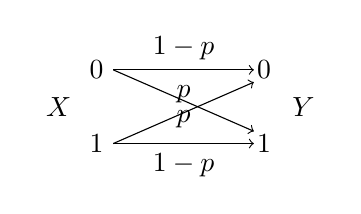
\begin{tikzpicture}[place/.style={inner sep=1pt}]
\matrix
{
    & \node(a1){0};  &    [18mm]     & \node[place](a2){0};        \\
\node{$X$}; &          &              &        &  \node{$\,\, Y$};            \\
    & \node(a3){1};  &             & \node[place](a4){1};        \\
};
\draw[->] (a1.east) --node[above]{$1-p$} (a2.west);
\draw[->] (a3.east) --node[above]{$p$} (a2.south west);
\draw[->] (a1.east) --node[below]{$p$} (a4.north west);
\draw[->] (a3.east) --node[below]{$1-p$} (a4.west);
\end{tikzpicture}
\end{center}
\caption{二进制对称信道}\label{fig:binary_symmetric_channel}%BSC
\end{figure}
使用“多数判决原则” 进行解码, 发生错误为 $(2n+1)$次传输有至少$n+1$次传错
$$p_e = \sum_{i = n+1}^{2n+1} \binom{2n+1}{i} p^i (1-p)^{2n+1-i}  $$
令 $ q = { p \over 1-p}\in (0,1)$,则
\begin{align*}
p_e & = \frac{q^{n+1} \sum_{j=0}^n q^j \binom{2n+1}{n-j}}{(1+q)^{2n+1}} \\
& \leq  \frac{q^{n+1} \sum_{j=0}^n  \binom{2n+1}{n-j}}{(1+q)^{2n+1}} \\
&  =  \frac{q}{1+q} \left(\frac{2\sqrt{q}}{1+q} \right)^{2n}
\end{align*}
因为$q\neq 1$, $\frac{2\sqrt{q}}{1+q}<1$ 所以当$n\to \infty$时,误码率$p_e \to 0$。

考虑二进制独立信源和对称信道,码率$R$和误码率 $P_e$ 的关系为:
$$
R \leq \frac{1-H(p)} {1-H(P_e)}
$$
\section{信道编码定理}
联合典型序列(Jointly Typical Sequence):
设 $(X, Y) \sim p(x,y)$, 随机序列对$(x^n, y^n) \in \X^n \times \Y^n $
是联合典型序列,当$x^n, y^n \in A^{(n)}_{\epsilon}$且 $\abs{-{1\over n} \log p(x^n, y^n) - H(X,Y)} <\epsilon$ 对给定的
$\epsilon$ 成立。

设 $\widetilde{X}^n$ 与 $\widetilde{Y}^n $ 独立,
$
\widetilde{X}^n \sim p(x^n), \widetilde{Y}^n \sim p(y^n) 
$
可以证明 
$$
 \Pr\{ (\widetilde{X}^n, \widetilde{Y}^n) \in A_{\epsilon}^{(n)}\} \leq  2^{-n (I(X;Y) - 3 \epsilon)} 
$$
因为
\begin{align*}
 \Pr\{ (\widetilde{X}^n, \widetilde{Y}^n) \in A_{\epsilon}^{(n)}\} & = 
\sum_{(x^n, y^n) \in A_{\epsilon}^{(n)}} p(x^n, y^n) \\
 & = 
\sum_{(x^n, y^n) \in A_{\epsilon}^{(n)}} p(x^n)p(y^n) \\
\end{align*}
由定义 $ p(x^n) \leq 2^{-n [H(x) - \epsilon]}, p(y^n) \leq 2^{-n [H(Y) - \epsilon]}$
所以
\begin{align*}
 \Pr\{ (\widetilde{X}^n, \widetilde{Y}^n) \in A_{\epsilon}^{(n)}\}  & \leq 
\sum_{(x^n, y^n) \in A_{\epsilon}^{(n)}}2^{-n [H(x)+H(Y) - 2\epsilon]}  \\
& = 2^{-n [H(x)+H(Y) - 2\epsilon]} \abs{A_{\epsilon}^{(n)}}
\end{align*}
由典型集的性质 $\abs{A_{\epsilon}^{(n)}} \leq 2^{n [H(X,Y) + \epsilon]} \Rightarrow$
\begin{align*}
 \Pr\{ (\widetilde{X}^n, \widetilde{Y}^n) \in A_{\epsilon}^{(n)}\}  & \leq 
2^{-n [ I(X; Y)-3\epsilon]} \\
\end{align*}
% shannon channel codeing theorem is omitted
\section{Hamming 码}
基本概念

所有码字 $c_i$ 的集合记为 一个码本 $C^{(n)} = \{ c_i \}_{i=1}^M $

码重: 二进制序列中 1 的个数, $ w(c_i) $

最小码重: $ w_{\min} = \min_{i} \{ w(c_i) \} $ (全零码除外)。

Hamming距离: 两个二进制序列中对应位不相等的个数, $ d(c_i, c_j ) $。

最小Hamming距离:$ d_{\min} = \min_{ i \neq j } \{ d(c_i, c_j) \} $。
\subsection{Hamming(7,4)}
4位数据位,3位校验位。 $d_{\min} = w_{\min} = 3 $。 码率 $ R = {4 \over 7}$。
顺序为 $ [p_1, p_2, d_1, p_3, d_2, d_3, d_4] $。其中 
\begin{align*}
 p_1 & = d_1 + d_2 + d_4 (\mathrm{mod} 2) \\
 p_2 & = d_1 + d_3 + d_4  (\mathrm{mod} 2) \\
 p_3 & = d_2 + d_3 + d_4  (\mathrm{mod} 2) \\
\end{align*}
生成矩阵$G$、解码矩阵 $ R$ 和校验矩阵 $H$ 具有下面的形式:
$$
G = \begin{bmatrix}
1 & 1 & 0 & 1 \\
1 & 0 & 1 & 1 \\
1 & 0 & 0 & 0 \\
0 & 1 & 1 & 1 \\
0 & 1 & 0 & 0 \\
0 & 0 & 1 & 0 \\
0 & 0 & 0 & 1
\end{bmatrix}
R = \begin{bmatrix}
0 & 0 & 1 & 0 & 0 & 0 & 0 \\
0 & 0 & 0 & 0 & 1 & 0 & 0 \\
0 & 0 & 1 & 0 & 0 & 1 & 0 \\
0 & 0 & 0 & 0 & 0 & 0 & 1
\end{bmatrix}
H = \begin{bmatrix}
1 & 0 & 1 & 0 & 1 & 0 & 1 \\
0 & 1 & 1 & 0 & 0 & 1 & 1 \\
0 & 0 & 0 & 1 & 1 & 1 & 1 
\end{bmatrix}
$$
\section{线性码}
将 $k$长的信息编码成$n$长的码字,生成矩阵$G$的维数是$n\times k$, 校验矩阵的
$H$的维数是 $(n-k) \times n$。
\subsection{循环码}
循环码是一类特殊的线性码,其编解码可通过生成多项式$g(x)$完成,$\degree(g(x)) = n-k$
设$g(x) = g_0 + g_1 x + \dots + g_{n-k} x^{n-k} $(共$n-k+1$ 个系数)

生成矩阵$G$的第$j$列是$x^{j-1}g(x)$的系数。

以二进制的$(7,4)$ 循环码为例,生成多项式整除$x^7 + 1 = (x+1)(x^3+x+1)(x^3+x^2+1)$。
取$g(x) = x^3 + x^2 + 1$,则生成矩阵为
$$
G = \begin{bmatrix}
1 & 0 & 0 & 0 \\
0 & 1 & 0 & 0 \\
1 & 0 & 1 & 0 \\
1 & 1 & 0 & 1 \\
0 & 1 & 1 & 0 \\
0 & 0 & 1 & 1 \\
0 & 0 & 0 & 1
\end{bmatrix}
$$
码字为如下16个(每行一个):
$$
\begin{array}{ccccccc}
0&0&0&0&0&0&0\\
0&0&0&1&0&1&1\\
0&0&1&0&1&1&0\\
0&0&1&1&1&0&1\\
0&1&0&1&1&0&0\\
0&1&0&0&1&1&1\\
0&1&1&1&0&1&0\\
0&1&1&0&0&0&1\\
1&0&1&1&0&0&0\\
1&0&1&0&0&1&1\\
1&0&0&1&1&1&0\\
1&0&0&0&1&0&1\\
1&1&1&0&1&0&0\\
1&1&1&1&1&1&1\\
1&1&0&0&0&1&0\\
1&1&0&1&0&0&1\\
\end{array}
$$
除全0和全1外,码重为3的7个码字和码重为4的7个码字为一组循环码。
校验多项式$h(x)g(x) = x^7 + 1 \Rightarrow h(x) = 1 + x^2 + x^3 + x^4 $。
校验矩阵$H$ 公式为
$$
H = \begin{bmatrix}
h_k & h_{k-1} & \dots & h_0 & 0 & \dots & 0 \\
0 & h_k & h_{k-1} & \dots & h_0 & \ddots & \vdots \\
\vdots & \ddots & \ddots & \ddots & & \ddots & & \\
0 & \dots & 0 & h_k & h_{k-1} & \dots & h_0 \\
\end{bmatrix}
$$
由此求出 
$$
H = \begin{bmatrix}
1 & 1 & 1 & 0 & 1 & 0  & 0 \\
0 & 1 & 1 & 1 & 0 & 1 & 0 \\
0 & 0 & 1 & 1 & 1 & 0 & 1 \\
\end{bmatrix}
$$
解码矩阵$RG=I_4 $,或求码字多项式$c(x)$除以$g(x)$的商的系数,此时仅利用了码字
最高4位进行解码,因此$R$ 的前3列均为0。由此解出 
$$ 
R = 
\begin{bmatrix}
0 & 0 & 0 & 1 & 1 & 1 & 0 \\
0 & 0 & 0 & 0 & 1 & 1 & 1 \\
0 & 0 & 0 & 0 & 0 & 1 & 1 \\
0 & 0 & 0 & 0 & 0 & 0 & 1 \\
\end{bmatrix}
$$
\subsection{系统码}
现要求码字以编码的信息为前缀,即码字对应的多项式中最高次项系数为消息。
设 $ p(x) $ 为表示消息的多项式, 一般的公式为
$ s_r(x) = p(x) x^{n-k} \mod g(x) $
将 $ s(x) = p(x) x^{n-k} - s_r(x) $ 作为码字。
对于我们选取的$(7, 4)$ 编码的例子, $ n = 7, k = 4$。 所以 求出 $$
G = \begin{bmatrix}
1 & 1 & 1 & 0 \\
0 & 1 & 1 & 1 \\
1 & 1 & 0 & 1 \\
1 & 0 & 0 & 0 \\
0 & 1 & 0 & 0 \\
0 & 0 & 1 & 0 \\
0 & 0 & 0 & 1
\end{bmatrix}
$$
\end{document}







